\documentclass[%
 reprint,
superscriptaddress,
%frontmatterverbose, 
%preprint,
%showpacs,preprintnumbers,
nofootinbib,
nobibnotes,
%bibnotes,
 amsmath,amssymb,
 aps,
%pra,
prd,
%rmp,
%prstab,
%prstper,
floatfix,
longbibliography
]{revtex4-1}


\usepackage{array}
\usepackage{amsmath}
\usepackage{float}
\usepackage{graphicx}
\usepackage{epstopdf}
%\usepackage{caption}
\usepackage[labelfont=bf,labelsep=period,justification=raggedright,singlelinecheck=false,font=small]{caption}
\renewcommand{\arraystretch}{1.5}
\usepackage{wrapfig}
\usepackage{verbatim}
\usepackage{amssymb}
\usepackage[normalem]{ulem}
\usepackage{hyperref}
%\usepackage[draft]{hyperref}
%\usepackage{times}
\usepackage[T1]{fontenc}
\usepackage[utf8]{inputenc}
\usepackage{comment}
\usepackage{multirow}
\usepackage{placeins} % For \FloatBarrier
\usepackage{subfigure}
\usepackage{threeparttable}
\usepackage{booktabs}
\usepackage{orcidlink}
%\usepackage{dblfloatfix}
\usepackage{dcolumn}% Align table columns on the decimal point
\usepackage{bm}% bold math
\usepackage[mathlines]{lineno}% Enable numbering of text and display math
\usepackage{tabularx}
\usepackage[export]{adjustbox}
\usepackage{url}
\usepackage{academicons}
\usepackage{xcolor}

\newcommand\Jc[1]{{\color{orange} \bf #1}} 

\newcommand\Add[1]{{\color{red} \bf #1}} %Newly Added words
\newcommand\Delete[1]{{\color{cyan} \bf #1}} %Prepared Deleted words

\newcommand{\sm}{\small}
\newcommand{\Rvir}{R_{\rm vir}}
\newcommand{\rvir}{R_{\rm vir}}
\newcommand{\mvir}{M_{\rm vir}}
\newcommand{\msun}{{\rm M}_{\odot}} 
\newcommand{\mstar}{{\rm M}_{*}}
\newcommand{\msunh}{h^{-1}{\rm M}_{\odot}} 
\newcommand{\mhalo}{M_{\rm h}}
\newcommand*{\lsim}{\mathord{\sim}}

\newif\ifshowfigures
\showfigurestrue


\hypersetup{
    pdfnewwindow=true,    % links in new window
    colorlinks=true,      % false: boxed links; true: colored links
    linkcolor=blue,       % color of internal links
    citecolor=blue,       % color of links to bibliography
    filecolor=blue,       % color of file links
    urlcolor=blue         % color of external links
}

\newcommand{\red}[1]{\textcolor{red}{#1}}
\newcommand{\blue}[1]{\textcolor{blue}{#1}}
\newcommand{\purple}[1]{\textcolor{purple}{#1}}
\newcommand{\yellow}[1]{\textcolor{yellow}{#1}}



\def\apj{ApJ}
\def\aap{A\& A}
\def\apjl{ApJL}
\def\apjs{ApJS}
\def\mnras{MNRAS}
\def\jcap{JCAP}
\def\pasa{PASA}
\def\aj{AJ}
\def\araa{ARA\& A}
\def\nat{Nature}
\def\prd{Phys. Rev. D}
\def\ssr{Space Sci. Rev.}
\def\rmxaa{RMxAA}
\def\na{New Astron}
\def \jqsrt{J. Quant. Spec. Radiat. Transf.}
\def \physrep{Phys. Rep.}
\def \pasj{PASJ} % "Publ. Astron. Soc. Jpn."

\newcommand\altaffilmark[1]{$^{#1}$}
\newcommand\altaffiltext[1]{$^{#1}$}



\begin{document}







\title{The Impact of Small-scale enhanced Primordial Power Spectrum on Nonlinear Structure Formation}

\author{Haina Huang\orcidlink{0009-0004-4765-0358}}
\thanks{\scriptsize \!\! Contact Author}
\email{hhuan155@link.cuhk.edu.hk} 
\affiliation{
 Department of Physics, The Chinese University of Hong Kong, Shatin, Hong Kong, China
}
\author{Tsang Keung Chan \orcidlink{0000-0003-2544-054X}}
\thanks{\scriptsize \!\! Contact Author}
\email{tsangkeungchan@cuhk.edu.hk}
\affiliation{
 Department of Physics, The Chinese University of Hong Kong, Shatin, Hong Kong, China
}
\author{Jianhao Wu \orcidlink{0009-0000-7431-7885}}
\thanks{\scriptsize \!\! Contact Author}
\email{jianhao.wu@wisc.edu}
\email{jianhao.wu@link.cuhk.edu.hk}
\affiliation{
 Department of Physics, University of Wisconsin-Madison, Madison, WI, USA
}
\affiliation{
 Department of Physics, The Chinese University of Hong Kong, Shatin, Hong Kong, China
}

\date{\today}







% ===== Abstract ===== #
\begin{abstract}
Motivated by the weak observational constraints on the primordial power spectrum at small scales, we use high-resolution dark-matter-only cosmological $N$-body simulations to quantify how enhanced small-scale primordial power is mapped into nonlinear structure formation. We compare a standard power-law primordial spectrum with two blue-tilted benchmark models that leave the large-scale spectrum unchanged while boosting power above a pivot wavenumber. For each model, we measure the halo mass function, half-mass assembly redshift, stacked halo density profiles, the concentration--mass relation, and the nonlinear matter power spectrum. We find that blue-tilted models produce a substantial excess of low-mass halos, especially at high redshift, and shift halo assembly to earlier times. At fixed mass, halos in the blue-tilted runs are systematically denser and more concentrated, with the strongest differences appearing in low-mass systems. The nonlinear matter power spectrum also develops a pronounced high-$k$ enhancement, showing that the primordial excess is amplified and redistributed by gravitational evolution. These results establish a controlled simulation-level benchmark for interpreting observational probes of small-scale primordial power, including JWST high-redshift galaxy counts, local dwarf-galaxy structure, strong-lensing substructure constraints, and future small-scale clustering measurements.
\end{abstract}

\maketitle

\section{Introduction\label{intro}}
The standard cosmological model, combining a nearly scale-invariant spectrum of primordial curvature perturbations with the $\Lambda$ Cold Dark Matter ($\Lambda$CDM) paradigm, provides an accurate description of the Universe on large scales. Measurements of the cosmic microwave background, galaxy clustering, and the Lyman-$\alpha$ forest are consistent with a red-tilted primordial power spectrum (PPS) over the range of scales that is directly constrained by current observations. The situation is less settled on smaller scales. Below the Mpc scale, the primordial spectrum is only weakly constrained, while the abundance and internal structure of low-mass halos remain central to long-standing small-scale questions such as the missing-satellites, core-cusp, and too-big-to-fail problems \citep{Bullock17smallscalechallenges,Sales22challenges}. At the same time, early JWST measurements have revealed unexpectedly abundant and potentially massive galaxy candidates at $z\gtrsim 8$--$10$ \citep{Labbe23MassiveGalaxies,Donnan23UVLF}, motivating renewed interest in whether modified small-scale initial conditions could accelerate early structure formation.

One economical way to test this possibility is to modify the PPS only on scales that are not already tightly fixed by CMB and large-scale structure data. A blue-tilted (BT) spectrum is a simple representative of this broader class of models. In this parametrization, the spectrum follows the usual red-tilted form on large scales, but changes slope above a pivot wavenumber $k_p$, so that modes with $k>k_p$ receive enhanced primordial power. Such a construction preserves the successful large-scale predictions of $\Lambda$CDM while directly changing the abundance and collapse history of small halos. More general possibilities include running spectral indices, broken power laws, localized features, primordial-black-hole motivated enhancements, or suppressed-power models; all of them ultimately ask how modified initial fluctuations are processed by nonlinear gravitational evolution.

Several recent studies have addressed different observational aspects of this question. Enhanced or modified small-scale spectra have been invoked to interpret high-redshift galaxy abundances in light of JWST \citep{Parashari23JWSTPPS,Hira24bluetilt}, and zoom-in simulations have explored the response of Milky Way--mass substructure to BT initial conditions \citep{Wu25BT}. Independent constraints can also come from dwarf-galaxy densities \citep{Dekker25DwarfPPS}, sub-galactic strong-lensing probes of the primordial matter power spectrum \citep{Gilman22SubgalacticPPS}, and 21 cm observations. In particular, the 21 cm signal has been proposed as a direct probe of otherwise inaccessible small-scale matter fluctuations during cosmic dawn and reionization \citep{Munoz20SmallScale21cm,deKruijf25DarkAges,Zhu26SKAPPS}. These works show that the same physical idea---changing the small-scale PPS---can be tested through several distinct observables, but they also highlight a key difficulty: galaxy formation, reionization, and observational selection effects can be degenerate with the primordial signal.

The purpose of this paper is to isolate the gravitational, nonlinear response to enhanced small-scale primordial power before adding those observation-specific complications. We therefore perform controlled dark-matter-only cosmological $N$-body simulations in periodic boxes, comparing a standard power-law PPS with two BT benchmark models. Rather than focusing on a single observable such as high-redshift galaxy counts or the substructure population of one Milky Way analog, we measure a set of complementary diagnostics: the halo mass function, half-mass assembly redshift, stacked halo density profiles, the concentration--mass relation, and the nonlinear matter power spectrum. These statistics probe different stages of the same physical process: enhanced small-scale fluctuations collapse earlier, populate the low-mass halo regime more efficiently, and are redistributed by nonlinear evolution into halo internal structure and high-$k$ clustering power.

This positioning is complementary to previous work. Studies of JWST galaxies ask whether enhanced small-scale power can help explain early luminous objects; 21 cm forecasts ask whether future surveys can detect the corresponding high-redshift signal; dwarf-galaxy and strong-lensing analyses ask how much deviation is still allowed at low redshift. Our work supplies the intermediate simulation-level link between the modified initial spectrum and the dark-matter statistics that underlie all of these observables. By mapping how the BT enhancement appears across multiple halo-based and field-level diagnostics, we identify which scales, masses, and epochs are most sensitive to the primordial modification and provide a benchmark for future forward modeling with baryons, survey selection, and likelihood analyses.


\section{Theoretical Overview}
\label{sec:theory}

This study investigates the imprints of a modified primordial power spectrum (PPS) on the late-time distribution of dark matter halos and subhalos. The theoretical framework connects the physics of the early universe, set during inflation, to the nonlinear structure formation observed today, and motivates the specific models we simulate.

\subsection{From Primordial Perturbations to Cosmic Structure}
The statistical properties of the density field in the late universe are seeded by quantum fluctuations amplified during the inflationary epoch. These initial conditions are characterized by the primordial power spectrum, $P_{\mathcal{R}}(k)$. In the standard $\Lambda$CDM cosmology, a nearly scale-invariant spectrum, $P_{\mathcal{R}}(k) \propto k^{n_s}$ with $n_s \approx 0.96$, is assumed. This spectrum undergoes linear evolution described by the transfer function $T(k)$ and growth factor $D(a)$ to yield the linear matter power spectrum, $P_{\mathrm{lin}}(k, a) \propto D^2(a) T^2(k) P_{\mathcal{R}}(k)$. The subsequent gravitational collapse and nonlinear evolution of overdensities lead to the formation of a hierarchical network of dark matter halos, whose internal structure and abundance serve as fundamental probes of the underlying cosmology.

\subsection{The Blue-Tilted Power Spectrum Model}
\yellow{As a first application of this broader program,} we consider a phenomenological extension to the standard PPS, the blue-tilted (BT) model, defined by a broken power-law form:
\begin{equation}
    P_i(k) \propto
    \begin{cases}
        k^{n_s}, & \left(\text{for } k < k_p\right),\\
        \left(\frac{k}{k_p}\right)^{m_s-n_s} k^{n_s}, & \left(\text{for } k > k_p\right),
    \end{cases}
\end{equation}
where $k_p$ is a pivot wavenumber and $m_s$ is the spectral index on scales $k > k_p$. This model preserves consistency with large-scale CMB and galaxy survey constraints ($k < k_p$), while enhancing power on smaller scales ($k > k_p$) when $m_s > n_s$ (blue tilt). The case $m_s < n_s$ corresponds to a red-tilted model. \yellow{Although the simulations in this paper focus on enhanced small-scale power, the analysis pipeline is intentionally phrased in terms of modified initial spectra: the same halo-based and field-level diagnostics can be used to test other PPS shapes once their initial conditions are generated consistently.}
\section{Numerical Methods}
\label{sec:numerical}

\subsection{Initial Conditions}
\blue{We generate the initial conditions with \textsc{Music2-MonofonIC}, adopting the Eisenstein \& Hu transfer function together with the primordial power spectra described in Section~\ref{sec:theory}. For the PL model, the primordial spectrum follows the standard power-law form. For the BT models, we replace the small-scale part of the spectrum with the broken power-law prescription in Eq.~(1), so that the large-scale modes remain unchanged while the power at $k>k_p$ is enhanced. In this way, the three simulation suites differ only in their primordial power spectra, enabling a controlled comparison of the resulting nonlinear structure formation.}
\subsection{Simulation Code}
\blue{We evolve the initial conditions with the cosmological $N$-body code \textsc{SWIFT}. In the dark-matter-only mode used here, \textsc{SWIFT} combines accurate short-range gravity with a long-range Particle Mesh treatment for periodic boxes, enabling efficient calculations over the full dynamic range of our simulations. Since all runs adopt the same numerical setup and background cosmology, the differences discussed in this paper can be attributed directly to the modified primordial power spectra rather than to changes in the gravity solver or simulation configuration.}
\subsubsection{Cosmological Parameters}
\label{subsub:cosmo_params}

For all the cosmological simulations in this paper, 

\begin{enumerate}
    \item Universe density parameters $\Omega_m=0.3153$, $\Omega_b=0.0493$, $\Omega_L= 0.6847$.
    \item Hubble constant $H_0 = 67.36 \ \rm{km}\ \rm{s}^{-1}\ \rm{cMpc}^{-1}$
    \item Scalar spectral index $n_s = 0.9649$
    \item Root-mean-square matter fluctuation averaged over a sphere of radius $8 h^{-1}~\rm{cMpc}$, $\sigma_8 = 0.8111$.
\end{enumerate}


\begin{table*}[t]
\centering
\small
\setlength{\tabcolsep}{4pt}
\renewcommand{\arraystretch}{1.25}
\begin{tabular}{l c c c c c c}
\hline
\hline
Model & $k_p$ & $m_s$ & $N$ & Box size & $m_{\text{DM}}$ & $\epsilon$ \\
 & $[h\,\text{Mpc}^{-1}]$ & & & $[h^{-1}\,\text{Mpc}]$ & $[h^{-1}M_\odot]$ & $[h^{-1}\,\text{Mpc}]$ \\
\hline
\textbf{Production Runs (N=1024)} \\
\hline
pl\_25\_1024   & -- & -- & $1024^3$ & 25 & $8.1\times 10^7$ & 0.000145 \\
kp\_1\_ms\_1.5\_25\_1024  & 1  & 1.5 & $1024^3$ & 25 & $8.1\times 10^7$ & 0.000145 \\
kp\_1\_ms\_2.0\_25\_1024  & 1  & 2.0 & $1024^3$ & 25 & $8.1\times 10^7$ & 0.000145 \\
kp\_10\_ms\_1.5\_25\_1024 & 10 & 1.5 & $1024^3$ & 25 & $8.1\times 10^7$ & 0.000145 \\
kp\_10\_ms\_2.0\_25\_1024 & 10 & 2.0 & $1024^3$ & 25 & $8.1\times 10^7$ & 0.000145 \\
kp\_1\_ms\_1.5\_5\_1024   & 1  & 1.5 & $1024^3$ & 5 & $1.3\times 10^6$ & 0.000029 \\
kp\_1\_ms\_1.5\_2.5\_1024 & 1  & 1.5 & $1024^3$ & 2.5 & $1.6\times 10^5$ & 0.0000145 \\

\hline
\textbf{Convergence Test Runs} \\
\hline
pl\_25\_512    & -- & -- & $512^3$  & 25 & $6.5\times 10^8$ & 0.00029 \\
pl\_25\_256    & -- & -- & $256^3$  & 25 & $5.2\times 10^9$ & 0.00058 \\
pl\_50\_512    & -- & -- & $512^3$  & 50 & $5.2\times 10^9$ & 0.00058 \\
pl\_256\_1024  & -- & -- & $1024^3$ & 256 & $1.4\times 10^{10}$ & 0.00148 \\
pl\_256\_512   & -- & -- & $512^3$  & 256 & $1.1\times 10^{11}$ & 0.00296 \\
\hline
\end{tabular}
\caption{Summary of cosmological N-body simulation parameters. PL models use standard power-law power spectra, while Blue Tilted models have enhanced power on small scales. $k_p$ is the wavenumber where the power spectrum enhancement begins, $m_s$ is the spectral index (tilt slope), $N$ is the number of dark matter particles, Box size is the comoving side length of the simulation volume, $m_{\text{DM}}$ is the dark matter particle mass, and $\epsilon$ is the gravitational softening length. All simulations use the same background cosmology with varying initial conditions to study the effects of small-scale power on structure formation.}
\label{tab:simulation_parameters}
\end{table*}



\subsection{Halo Finder and Halo Property Post-processor}
\blue{In the main text, halos and merger trees are identified with \textsc{HBT+}, a particle-tracking halo finder well suited to following bound structures and their progenitors across snapshots. We require a minimum of 20 particles for an object to be retained as a halo candidate. The halo center is defined as the position of the most bound particle. Based on the \textsc{HBT+} catalogs, we then use \textsc{SOAP} (Spherical Overdensity and Aperture Processor) to compute spherical-overdensity properties such as $M_{200c}$, $R_{200c}$, and the corresponding structural quantities used below. This separation between halo identification and property measurement allows us to retain the tracking information from \textsc{HBT+} while adopting a consistent spherical-overdensity definition for the profile and concentration analyses.}


\subsection{Simulation Suite and Terminology\label{subsec:Terminology}}
We run nine simulations using the numerical pipeline described above. Their numerical settings are listed in Table~\ref{tab:simulation_parameters}. The six fiducial-resolution simulations are used to compare the BT and the PL models. In the discussion below, we use PL to denote the standard power-law primordial power spectrum, while BT\_soft and BT\_deep denote the two blue-tilted variants adopted for the main comparisons.

\subsection{Numerical Robustness and Convergence}
\begingroup
\color{red}
To assess the numerical robustness of the main results, we performed a set of convergence tests spanning both mass resolution and box size, as summarized in Table~\ref{tab:simulation_parameters}. These tests are intended to establish the ranges over which the halo abundance, internal structure, and clustering statistics are numerically reliable, and to distinguish physical trends caused by the modified primordial power spectrum from numerical artifacts. In practice, three classes of effects are particularly important: particle discreteness at the low-mass end, finite-volume suppression at the high-mass and large-scale ends, and force-softening effects in the inner regions of halos.

For halo abundance statistics, the most conservative limitation arises from the minimum number of particles required to define a robust object. Although we retain halo candidates above 20 particles in the catalog construction, the scientific interpretation of the halo mass function is restricted to a higher effective threshold, because quantities such as the FOF mass and derived abundance become increasingly sensitive to discreteness and halo-finding noise near the formal detection limit. Our fiducial analysis therefore focuses on the mass interval where the production runs and the convergence-test runs show qualitatively stable behavior under changes in resolution. Similarly, the high-mass end is limited by the finite simulation volume, which reduces the number of rare objects and amplifies sample variance.

For internal halo structure, convergence is more restrictive in radius than in total mass. The density profile and concentration measurements are expected to be most sensitive to force softening, particle number, and centering uncertainties in the inner halo. Accordingly, the trends emphasized in the main text should be interpreted as robust only outside the innermost numerically unresolved region and for halo masses that are sufficiently well sampled by particles. In future revisions, these limits will be quantified explicitly using resolution-comparison panels and radial convergence criteria. The present analysis should therefore be viewed as establishing the qualitative and intermediate-scale structural response of halos to blue-tilted initial conditions, rather than claiming percent-level convergence at the smallest radii.

For the nonlinear matter power spectrum, the usable dynamic range is bounded on large scales by the simulation box size and on small scales by force resolution, particle sampling, and grid-assignment effects in the power-spectrum estimator. The interpretation of the highest-$k$ bins should therefore be understood as indicative of a strong enhancement trend rather than as a precision measurement at arbitrarily small scales. A full production version of this paper should include an explicit summary table of the trusted mass, radius, and wavenumber intervals adopted for each statistic.
\endgroup

\section{Results}
\label{sec:results}

We compare the PL, BT\_deep, and BT\_soft simulations in the following order: the initial power spectrum, the projected simulation maps, the halo mass function, the half-mass redshift, the halo profiles, and the nonlinear power spectrum.

\subsection{Initial Power Spectrum}
We focus on two specific BT models, with parameters adopted from previous BT studies on JWST early massive galaxies \cite{Hira24bluetilt} and enhancing MW substructures \citep{Wu25BT}:
\begin{itemize}
    \item \textbf{BT\_soft}: A model with a relatively low pivot scale ($k_p \approx 1.0$ Mpc$^{-1}$) and moderate enhancement ($m_s \approx 1.5$).
    \item \textbf{BT\_deep}: A model with a higher pivot scale ($k_p \approx 10$ Mpc$^{-1}$) and similar spectral tilt.
\end{itemize}
These two models allow us to explore the scale dependence of the BT modification's effects. For comparison, we also simulate the standard power-law (PL) model ($m_s = n_s$), which serves as our baseline.

\ifshowfigures
\begin{figure}[tp]
    \centering
    
\includegraphics[width=\columnwidth]{input-power-spectrum.png}
    \caption{\blue{Illustrative comparison of the initial matter power spectra for the primordial models considered in this work. The figure shows how changing the small-scale tilt and pivot scale modifies the power spectrum only at high wavenumber, while leaving the large-scale behavior close to the standard power-law form. This localized enhancement at $k>k_p$ defines the BT models and sets the initial conditions for the subsequent nonlinear evolution.}}
    \label{fig:power_spectrum_comparison}
\end{figure}
\fi

\begin{table}[t]
\centering
\begin{tabular}{@{}lll@{}}
\toprule
           \multicolumn{1}{l}{Models}
           &
           \multicolumn{2}{c}{Related parameters} \\ \midrule
PL &  \multicolumn{2}{c}{Power Law Primordial Power Spectrum}    \\
& $n_s=0.961$ \\

BT\_deep &    $k_p = 3.51 \ \rm{cMpc}^{-1}$ & $ m_s = 1.5$   \\
BT\_soft &    $k_p = 0.702 \ \rm{cMpc}^{-1}$ & $ m_s = 1.5$   \\

\bottomrule

\end{tabular}
\caption{The parameters of all the chosen models. $k_p$ is the wave vector at which the BT PPS would deviate from the PL PPS. $m_s$ is the enhanced spectral index for $k>k_p$, at the small scales. For other cosmological parameters, see \protect\autoref{subsub:cosmo_params}.}
\label{tab:Params_all_models}
\end{table}

\subsection{Simulation Maps}
The projected dark matter distribution maps from the PL, BT\_deep, and BT\_soft simulations show that the main halos remain broadly similar in projection. However, the BT model contains a significantly larger number of subhalos than the PL model, including both small and massive subhalos. In terms of spatial distribution, the substructures in the BT model are also more centrally concentrated compared to those in the PL model.

\ifshowfigures
\begin{figure*}[t]
    \centering
    \includegraphics[width=0.86\textwidth,height=0.68\textheight,keepaspectratio]{projection.png}
    \caption{\blue{Projected dark matter density fields for the PL, BT\_soft, and BT\_deep simulations at $z=0$. All three runs use a periodic box of $25\,h^{-1}\,\mathrm{Mpc}$ with $1024^3$ particles. The large-scale structure remains similar among the models, whereas the blue-tilted runs exhibit visibly richer small-scale substructure, consistent with the enhancement of primordial power at $k>k_p$.}}
    \label{fig:dark_matter_comparison}
\end{figure*}
\fi

\subsection{Halo Mass Function\label{subsub:HMF}}
We utilize a set of high-resolution cosmological simulations to investigate the evolution of the halo mass function from high redshift (approximately $z \approx 8.5$) to the present day, aiming to place constraints on models featuring a blue-tilted primordial power spectrum. The analysis is based on three representative cosmological simulation models: the PL model employing a standard power-law power spectrum serves as the baseline, while two blue-tilted power spectrum models with differing tilt strengths (BT\_hard and BT\_soft) are used for comparative study. To trace the history of structure formation, we sampled at nine distinct epochs from high to low redshift (corresponding to snapshot numbers 32 to 56).

\ifshowfigures
\begin{figure*}[t]
    \centering
    
\includegraphics[width=0.90\textwidth,height=0.72\textheight,keepaspectratio]{mass-function.png}
    \caption{\blue{Halo mass functions for the PL, BT\_soft, and BT\_deep models at representative redshifts between $z\approx 8.5$ and $z=0$. Symbols show the simulation results and lines show the corresponding analytic expectations. The blue-tilted models predict a clear excess of low-mass halos relative to PL, particularly at high redshift, while the differences decrease toward the high-mass end and at later times.}}
    \label{fig:mass_function}
\end{figure*}
\fi

Halo masses are defined using the \textbf{Friends-of-Friends (FOF)} algorithm, which links dark matter particles into halos via a given linking length (typically 0.2 times the mean particle separation). These FOF halo masses are extracted from the post-processing catalogs generated by the \textsc{SWIFT} simulation. \blue{To minimize binning noise, we evaluate the halo mass function with an integration-averaging procedure rather than a simple count-per-bin histogram.} We partition the mass range in logarithmic space with a density of six bins per mass decade. Within each bin, we compute the integral of the halo count and the mass-weighted average mass. The mass function $\frac{dn}{d\log M}$ is calculated via:
\begin{equation}
\frac{dn}{d\log M} = \frac{\int dn}{V \cdot \Delta \log M}.
\end{equation}
Statistical errors are estimated based on Poisson statistics, given by $\sigma = \sqrt{N}/(V \cdot \Delta \log M)$, where $N$ is the number of halos in the bin. The volume of the periodic simulation box is $(25\ \mathrm{Mpc}/h)^3$. \blue{At the low-particle end, raw FOF masses are known to be biased high because discreteness effects artificially inflate the measured halo size. To reduce this bias, we apply the Warren correction \protect\cite{Warren_2006},}
\begin{equation}
\blue{N_{\text{corrected}} = N(1-N^{-0.6}),}
\end{equation}
\blue{before converting particle number to physical halo mass. After this correction, we keep halos in the range $10^{8}$--$10^{13}\,M_\odot$, corresponding to the mass interval where the combination of particle resolution and box statistics remains reliable for our fiducial runs.}

For theoretical comparison, we compute predictions using the \textsc{Colossus} cosmology package. To ensure a fair comparison, we extended the Colossus package by implementing three new custom power spectrum models: \texttt{eisenstein98\_bt}, \texttt{eisenstein98\_bt\_soft}, and \texttt{eisenstein98\_pl}. These models are built upon the well-established Eisenstein \& Hu (1998) transfer function but incorporate a segmented primordial power spectrum designed to produce a blue tilt on small scales. The core modification involves introducing a transition wavenumber $k_p$, beyond which the primordial spectral index shifts from the large-scale value $n_s$ to an enhanced value $m_s$.

Special attention was paid to numerical stability during the implementation of these models, ensuring the positivity of the power spectrum and handling potential overflow or underflow issues in the power-law calculations. Theoretical calculations strictly adopt the initial power spectrum matching each simulation model and specify the halo mass definition consistent with the simulations (i.e., selecting the parameter \texttt{mdef='fof'}). \blue{For the analytic comparison, we use the standard multiplicity-function framework,}
\begin{equation}
\blue{\frac{dn}{d\ln M} = \frac{\bar{\rho}_{\rm m}}{M} f(\sigma)\left|\frac{d\ln \sigma^{-1}}{d\ln M}\right|,}
\end{equation}
\blue{where $\bar{\rho}_{\rm m}$ is the mean matter density, $\sigma(M)$ is the linear variance of the smoothed density field, and $f(\sigma)$ is the fitting function calibrated from simulations. In practice, we adopt the fitting formula from \protect\cite{Reed_2007}, evaluated using the linear power spectrum corresponding to each primordial model and then converted into physical units consistent with the simulation data.}

To quantify the differences between simulations and theory, we performed a detailed comparison. The theoretical curve is aligned to the mass positions of the simulation data points via one-dimensional interpolation, and the relative difference in each mass bin is calculated:
\begin{equation}
\Delta = \frac{f_{\mathrm{sim}}(M) - f_{\mathrm{theory}}(M)}{f_{\mathrm{theory}}(M)},
\end{equation}
where $f(M) = dn/d\log M$ is the mass function. The statistical errors from the simulations are propagated accordingly into the differences.

The halo mass-function comparison across nine redshifts shows that, at the low-mass end and especially at high redshift ($z > 5$), the simulation results for the blue-tilted models significantly exceed the theoretical predictions of the standard model. Therefore, we can utilize the behavior of the mass function at the low-mass end to discriminate between different primordial power spectrum models. The predictions of the strong blue-tilt model and the standard model gradually converge at the high-mass end, consistent with their behavior on scales dominated by nonlinear evolution. Meanwhile, the predictions of the weak blue-tilt model lie between the two across the entire mass range, consistent with its moderate modification of the power spectrum.

The reliable range of the mass function is determined by the simulation volume and resolution limits. In the middle and lower sub-panels (corresponding to intermediate and low redshift, $z < 5$), within the statistically reliable range, the strong blue-tilt model consistently exhibits a higher abundance than the standard model at the low-mass end ($M < 10^{10} M_{\odot}$), while at the high-mass end ($M > 10^{11} M_{\odot}$), the predictions of all models gradually converge. This is also consistent with our theoretical expectation that blue-tilted models primarily affect small-scale structure. As redshift decreases, the differences between model predictions at the high-mass end gradually diminish, indicating that the formation of massive halos at late times is predominantly governed by later-stage nonlinear evolution.

\subsection{Half-Mass Redshift\label{subsub:HMR}}
We compare the redshift at which halos reach half of their final mass ($z_{1/2}$) as a function of their $z=0$ mass for three cosmological models: standard CDM (PL), the strongly blue-tilted model (BT, $k_p=1$), and the weakly blue-tilted model (BT, $k_p=10$). This quantity, also known as the half-mass epoch, serves as a fundamental indicator of halo assembly history, characterizing when the bulk of a halo's final mass was accreted. Our analysis is based on the mass evolution tracks of individual halos extracted from HBT+ halo merger trees across four initial mass bins spanning $10^{-3}$ to $10^{1}$ in units of $10^{10} M_{\odot}$.

\ifshowfigures
\begin{figure*}[t]
    \centering
    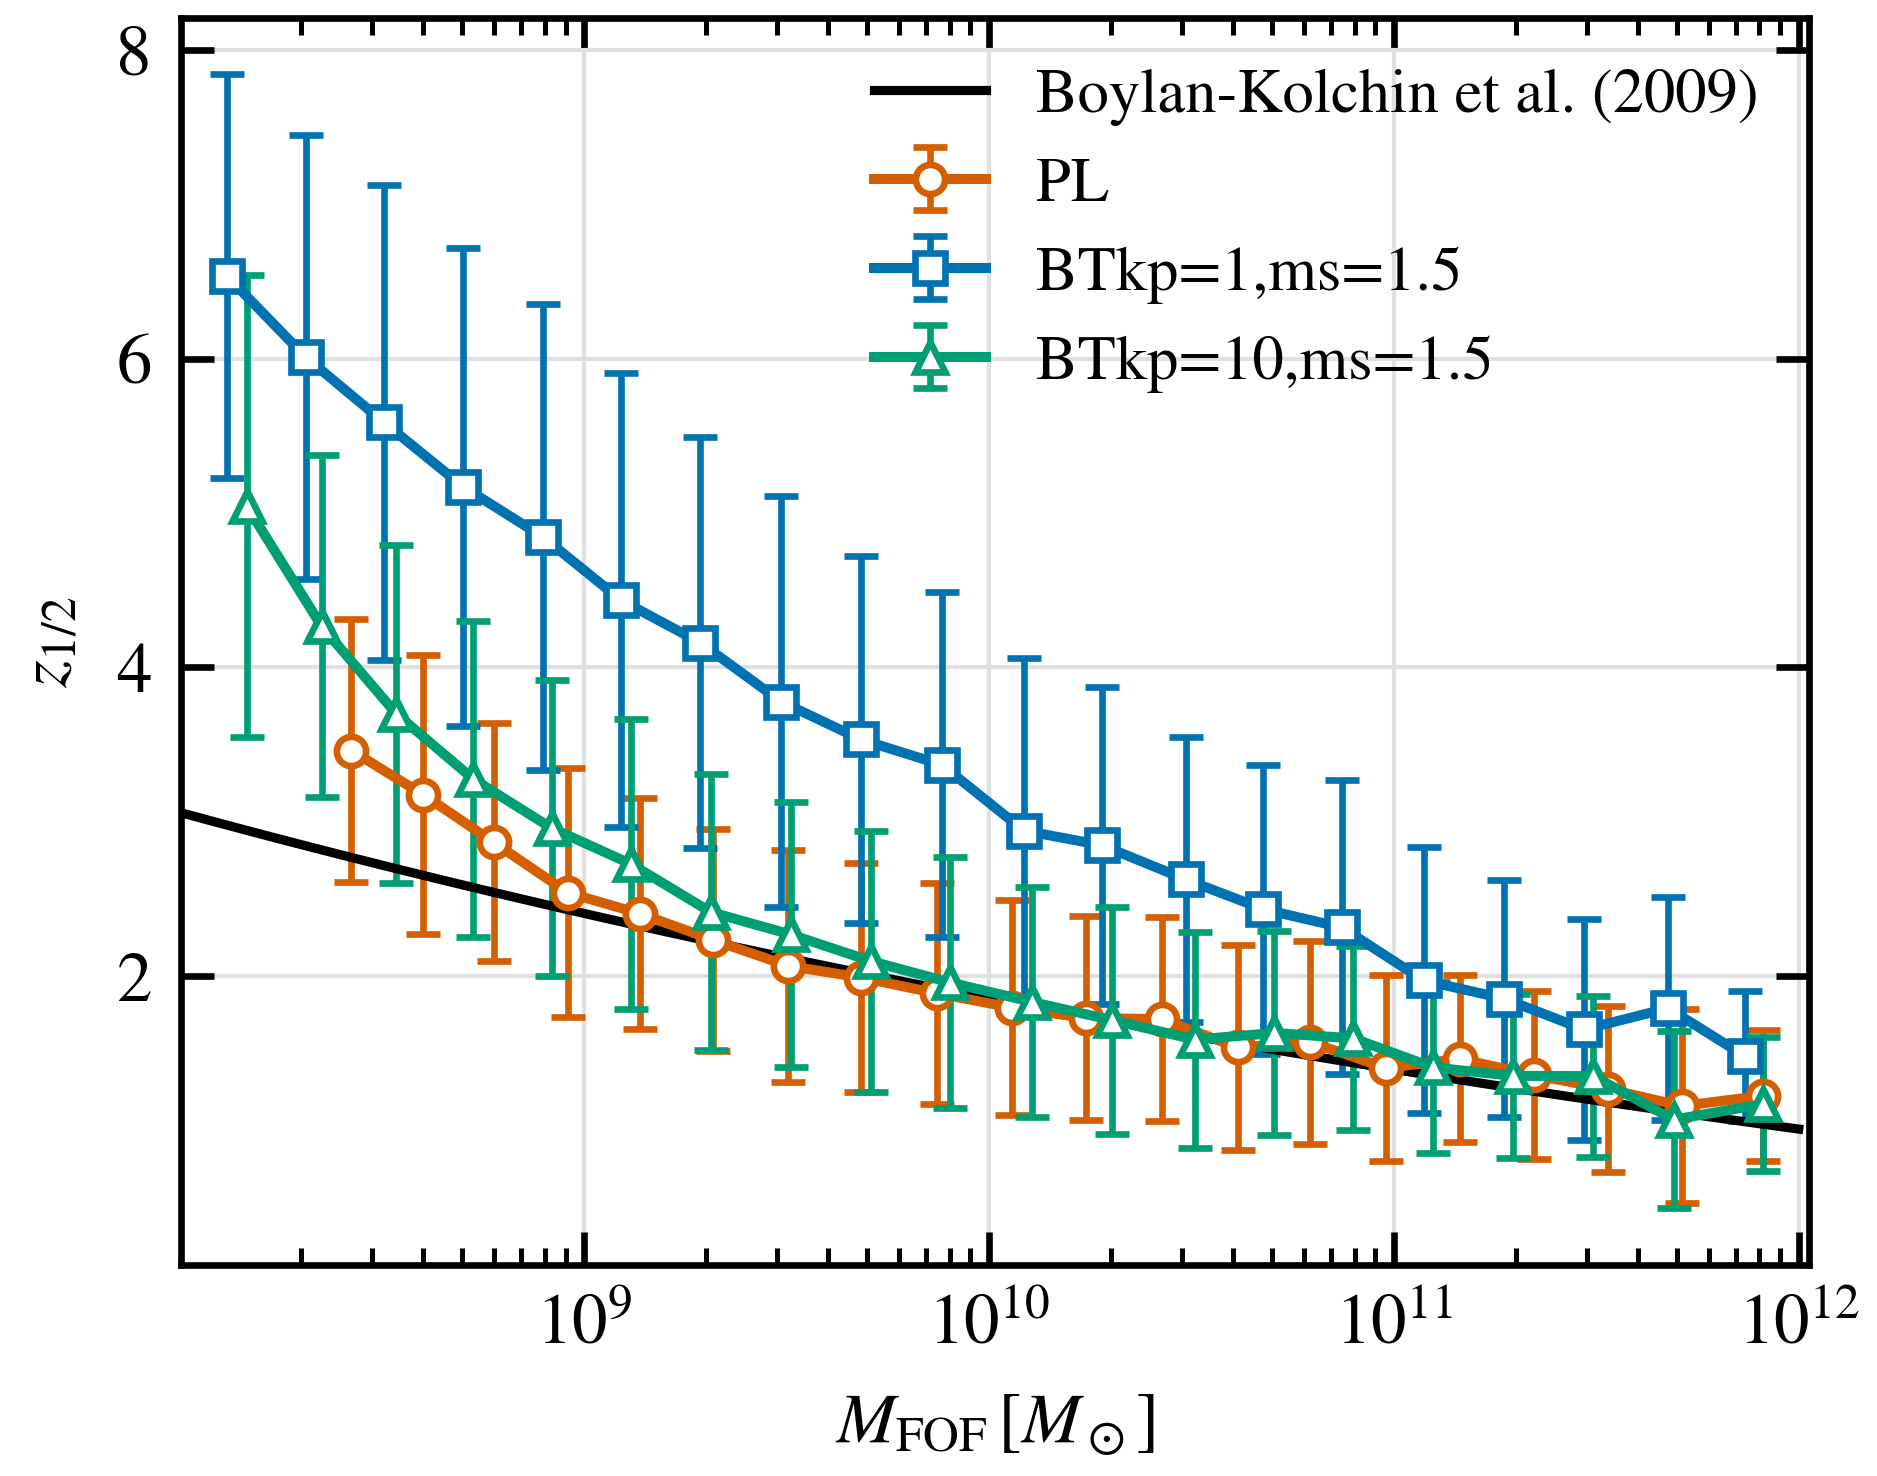
\includegraphics[width=0.88\textwidth,height=0.66\textheight,keepaspectratio]{halfmass-redshift.png}
    \caption{\blue{Half-mass assembly redshift $z_{1/2}$ as a function of halo mass at $z=0$ for the PL, BT\_soft, and BT\_deep simulations. Each point gives the mean $z_{1/2}$ of halos in a mass bin, where $z_{1/2}$ is defined from the main progenitor branch of the merger tree; error bars indicate the standard deviation within the bin. Halos in the blue-tilted models reach half of their final mass systematically earlier than their PL counterparts, especially at intermediate masses.}}
    \label{fig:half_mass_redshift}
\end{figure*}
\fi

The computation of $z_{1/2}$ follows a robust methodology: for each halo, we first determine its mass at $z=0$ ($M_{z=0}$). \blue{We then follow the mass of its main progenitor branch backward in time through 21 discrete redshift outputs (from $z=0$ to $z\approx8.5$), and linearly interpolate between adjacent snapshots to identify the redshift at which the main progenitor first reaches $M_{z=0}/2$.} Halos that do not reach half of their final mass within the redshift range are excluded from the analysis.

To establish the mass dependence of the assembly history, halos are partitioned into distinct mass bins based on their $z=0$ mass in logarithmic space. The lowest mass bin ($10^{-3}$ to $10^{-2} \times 10^{10} M_{\odot}$) is treated as a single partition due to limited statistics, while each of the three higher mass bins is subdivided into five equally spaced logarithmic sub-bins. For each resulting mass bin, we compute the mean and standard deviation of $z_{1/2}$ across all member halos.

The comparison reveals a clear mass-dependent assembly trend across all models: low-mass halos ($M_{z=0} \lesssim 10^{9} M_{\odot}$) assemble the majority of their mass earlier (higher $z_{1/2}$) compared to their high-mass counterparts ($M_{z=0} \gtrsim 10^{10} M_{\odot}$), consistent with hierarchical structure formation. However, the blue-tilted models exhibit systematic offsets relative to the standard CDM model. The strongly blue-tilted model (BT, $k_p=1$) shows the highest $z_{1/2}$ values across nearly all mass bins, indicating that halos in this model assemble their mass earlier. The weakly blue-tilted model (BT, $k_p=10$) generally falls between the other two models, though it approaches the standard CDM predictions at the highest masses. These differences are most pronounced at intermediate masses ($M_{z=0} \sim 10^{9} - 10^{10} M_{\odot}$), where the enhanced small-scale power in blue-tilted models promotes earlier halo formation and mass assembly.
This systematic shift in assembly history provides complementary evidence for the impact of blue-tilted primordial power spectra on structure formation, independent of halo abundance and density profile analyses. The earlier assembly of halos, particularly at intermediate masses, may have significant implications for the formation timescales of galaxies and the thermal history of the intergalactic medium in these models.

\subsection{Halo Profiles}
\subsubsection{Halo Density Profile\label{subsub:DensityProfile}}
Based on the analysis of our simulation data, we systematically compare the density profiles of dark matter halos across the standard Cold Dark Matter (CDM) model, the strongly blue-tilted model ($k_p=1$), and the weakly blue-tilted model ($k_p=10$). The results indicate that the internal structure of halos is highly sensitive to the blue-tilted modification of the primordial power spectrum, and its response exhibits a significant radial dichotomy and mass dependence.

\ifshowfigures
\begin{figure*}[t]
    \centering
    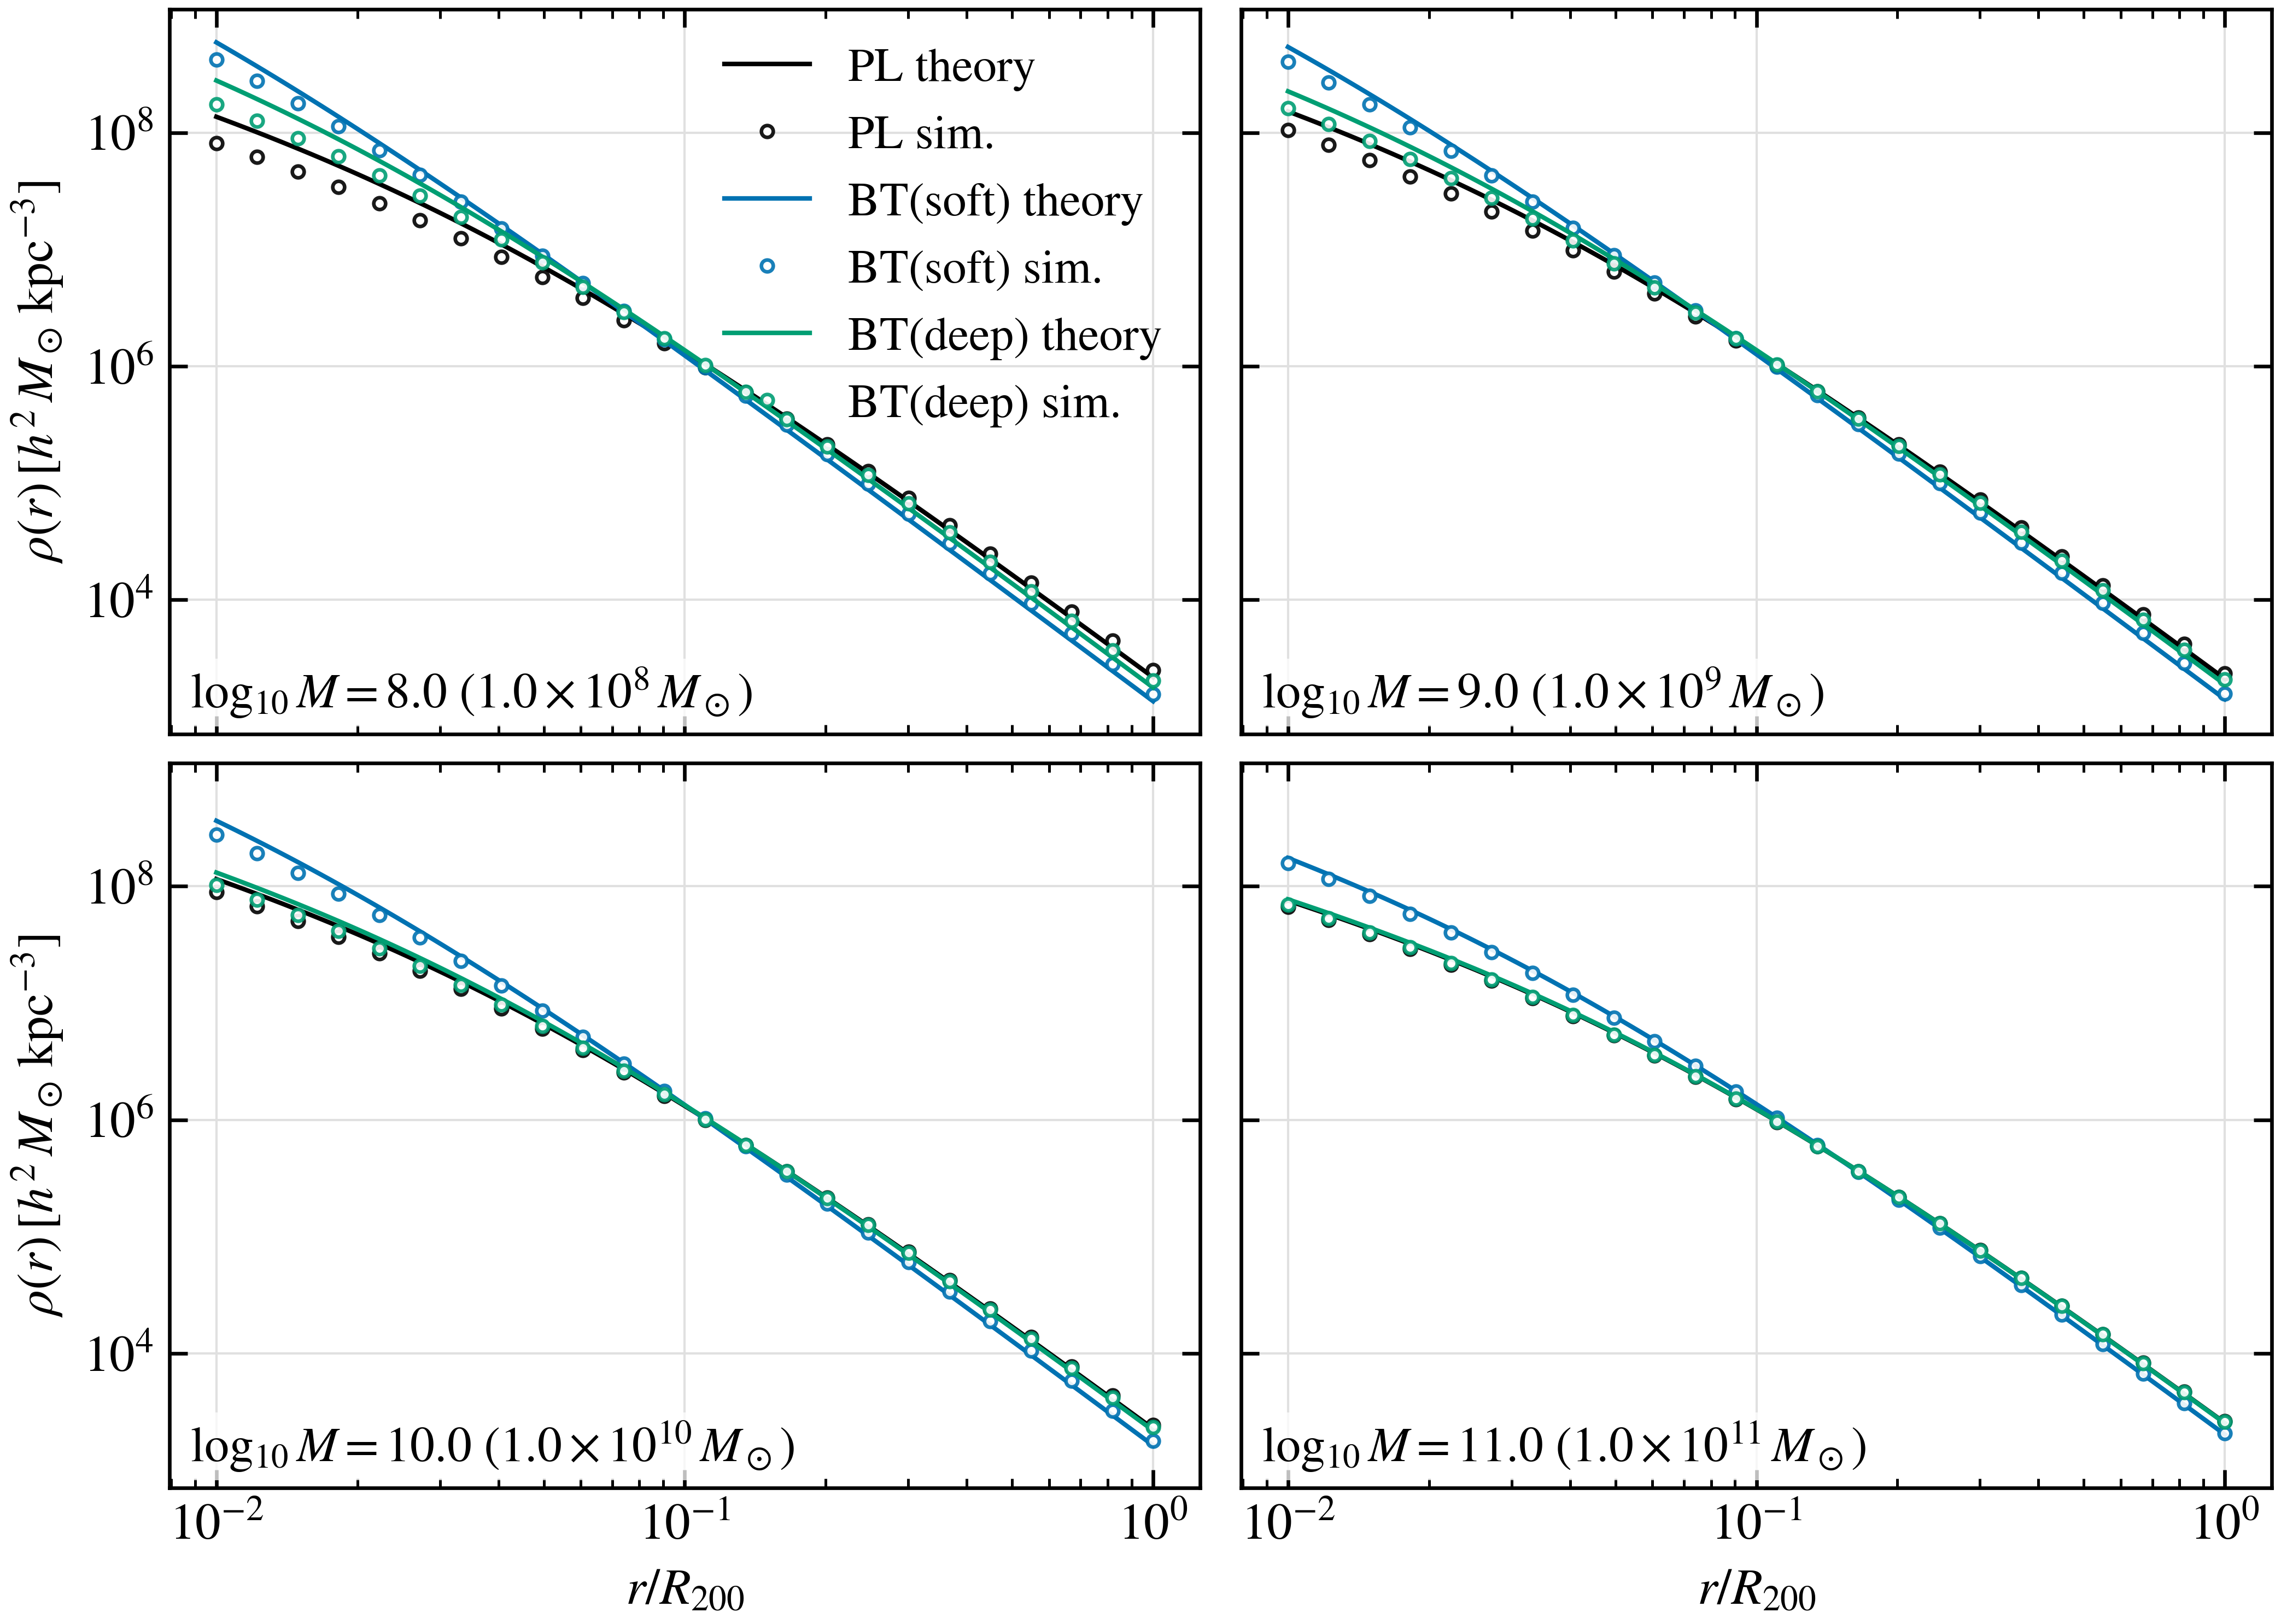
\includegraphics[width=0.92\textwidth,height=0.66\textheight,keepaspectratio]{halo-density.png}
    \caption{\blue{Stacked halo density profiles for the PL, BT\_soft, and BT\_deep models in a sequence of halo-mass bins. Radii are normalized by $R_{200}$, and each panel compares halos within a narrow mass interval. Relative to PL, the blue-tilted models exhibit higher central densities, with the strongest effect appearing in the low- and intermediate-mass regimes.}}
    \label{fig:halo_density_analysis}
\end{figure*}
\fi

In the inner regions ($r < 0.1, R_{200}$), the strongly blue-tilted model ($k_p=1$) shows the most pronounced density enhancement across almost the entire mass range, followed by the weakly blue-tilted model ($k_p=10$), while the CDM model predicts the lowest central density. This suggests that the extra power on small scales in the blue-tilted power spectrum efficiently promotes the early collapse and mass concentration in the halo cores.

In the outer regions ($r > 0.3, R_{200}$), the differences between models display a clear evolution with mass. For high-mass halos ($M_h \gtrsim 10^{12} M_\odot$), the density profiles of all three models converge and are nearly indistinguishable. Moving into the intermediate mass range ($10^9 \lesssim M_h \lesssim 10^{11} M_\odot$), the outer density of the strongly blue-tilted model begins to fall systematically below that of the CDM and weakly blue-tilted models, with this density deficit increasing progressively as the halo mass decreases. At the low-mass end ($M_h \lesssim 10^8 M_\odot$), the behavior of the three models becomes distinctly stratified: the strongly blue-tilted model exhibits the most extreme signature of high inner density coupled with low outer density; the weakly blue-tilted model shows intermediate densities at all radii; whereas the CDM model is characterized by the lowest inner density but the relatively highest outer density.
This unique radial anti-correlation---inner enhancement paired with outer suppression---reveals that the blue-tilted modification not only directly affects the early formation and central collapse of halos by enhancing small-scale power but also modulates their subsequent mass accretion history in a complex, mass-dependent manner. The systematic reduction of outer density in intermediate and low-mass halos may be linked to the increased subhalo abundance, and differences in the large-scale matter distribution in blue-tilted models, the specific mechanisms of which warrant further investigation. These findings provide a novel theoretical perspective for using the global density structure of halos to precisely discriminate between and constrain different models of the primordial power spectrum.

\subsubsection{Concentration-Mass Relation\label{subsub:concentration}}
The concentration--mass relation is derived from halo catalogs generated by the \textsc{hbt+} halo finder applied to the outputs of the Blue-tilted and CDM simulations. We extract the halo mass \(M_{200c}\) and the corresponding concentration \(c_{200c}\) from the \texttt{SO/200\_crit} group of the HDF5 file. The masses are converted to solar masses by multiplying the stored values by the unit factor \(10^{10}\,M_{\odot}\). Only halos with positive masses are retained, and the mass is transformed to logarithmic scale, \(\log_{10}(M_{200c}/M_{\odot})\).

To characterize the median concentration as a function of mass, we bin the halos in logarithmic mass bins. The mass range from \(\log_{10}(M/M_{\odot}) = 8.0\) to \(13.5\) is divided into 100 equally spaced bins. Within each bin, we compute the median concentration as well as the 16th and 84th percentiles. The lower and upper error bars for the median are then defined as \(\mathrm{median} - P_{16}\) and \(P_{84} - \mathrm{median}\), respectively. These percentiles provide an estimate of the scatter in the concentration--mass relation.

Theoretical predictions for the concentration--mass relation are obtained using the \textsc{colossus} Python package \citep{Diemer2018}. We adopt two widely used models: the Diemer \& Joyce (2019) model \citep{Diemer2019} and the Ishiyama et al. (2021) model \citep{Ishiyama2021}. For each model, we compute the median concentration at the same redshifts as the simulation snapshots. The models require an input mass definition of \(M_{200c}\), which we adopt. Additionally, the power spectrum used in the model is specified via the \texttt{ps\_args} parameter. To match the two cosmological scenarios, we employ two different power spectra: the Eisenstein \& Hu (1998) transfer function \citep{Eisenstein1998} with the default power-law primordial spectrum (\texttt{eisenstein98\_pl}) for the CDM case, and a modified version with a blue-tilted primordial spectrum (\texttt{eisenstein98\_bt}) for the Blue-tilted simulation. The cosmological parameters are set consistently with the simulations: \(H_0 = 67.36\ \mathrm{km\,s^{-1}\,Mpc^{-1}}\), \(\Omega_m = 0.3153\), \(\Omega_b = 0.0493\), \(\sigma_8 = 0.8111\), and \(n_s = 0.9649\). The theoretical curves are then plotted over the same mass range as the binned simulation data, allowing a direct comparison between the simulated concentration--mass relations and the analytic predictions.
\blue{In these analytic models, the concentration is not fitted independently in each mass bin; instead, it is predicted from the collapse history encoded in the linear density field. The underlying assumption is that halo concentration is primarily determined by the characteristic density of the Universe at the epoch when the inner part of the halo assembled. As a result, once the linear power spectrum and cosmological parameters are specified, the concentration--mass relation can be predicted semi-analytically and compared directly with the simulation output.}

\ifshowfigures
\begin{figure*}[t]
    \centering
    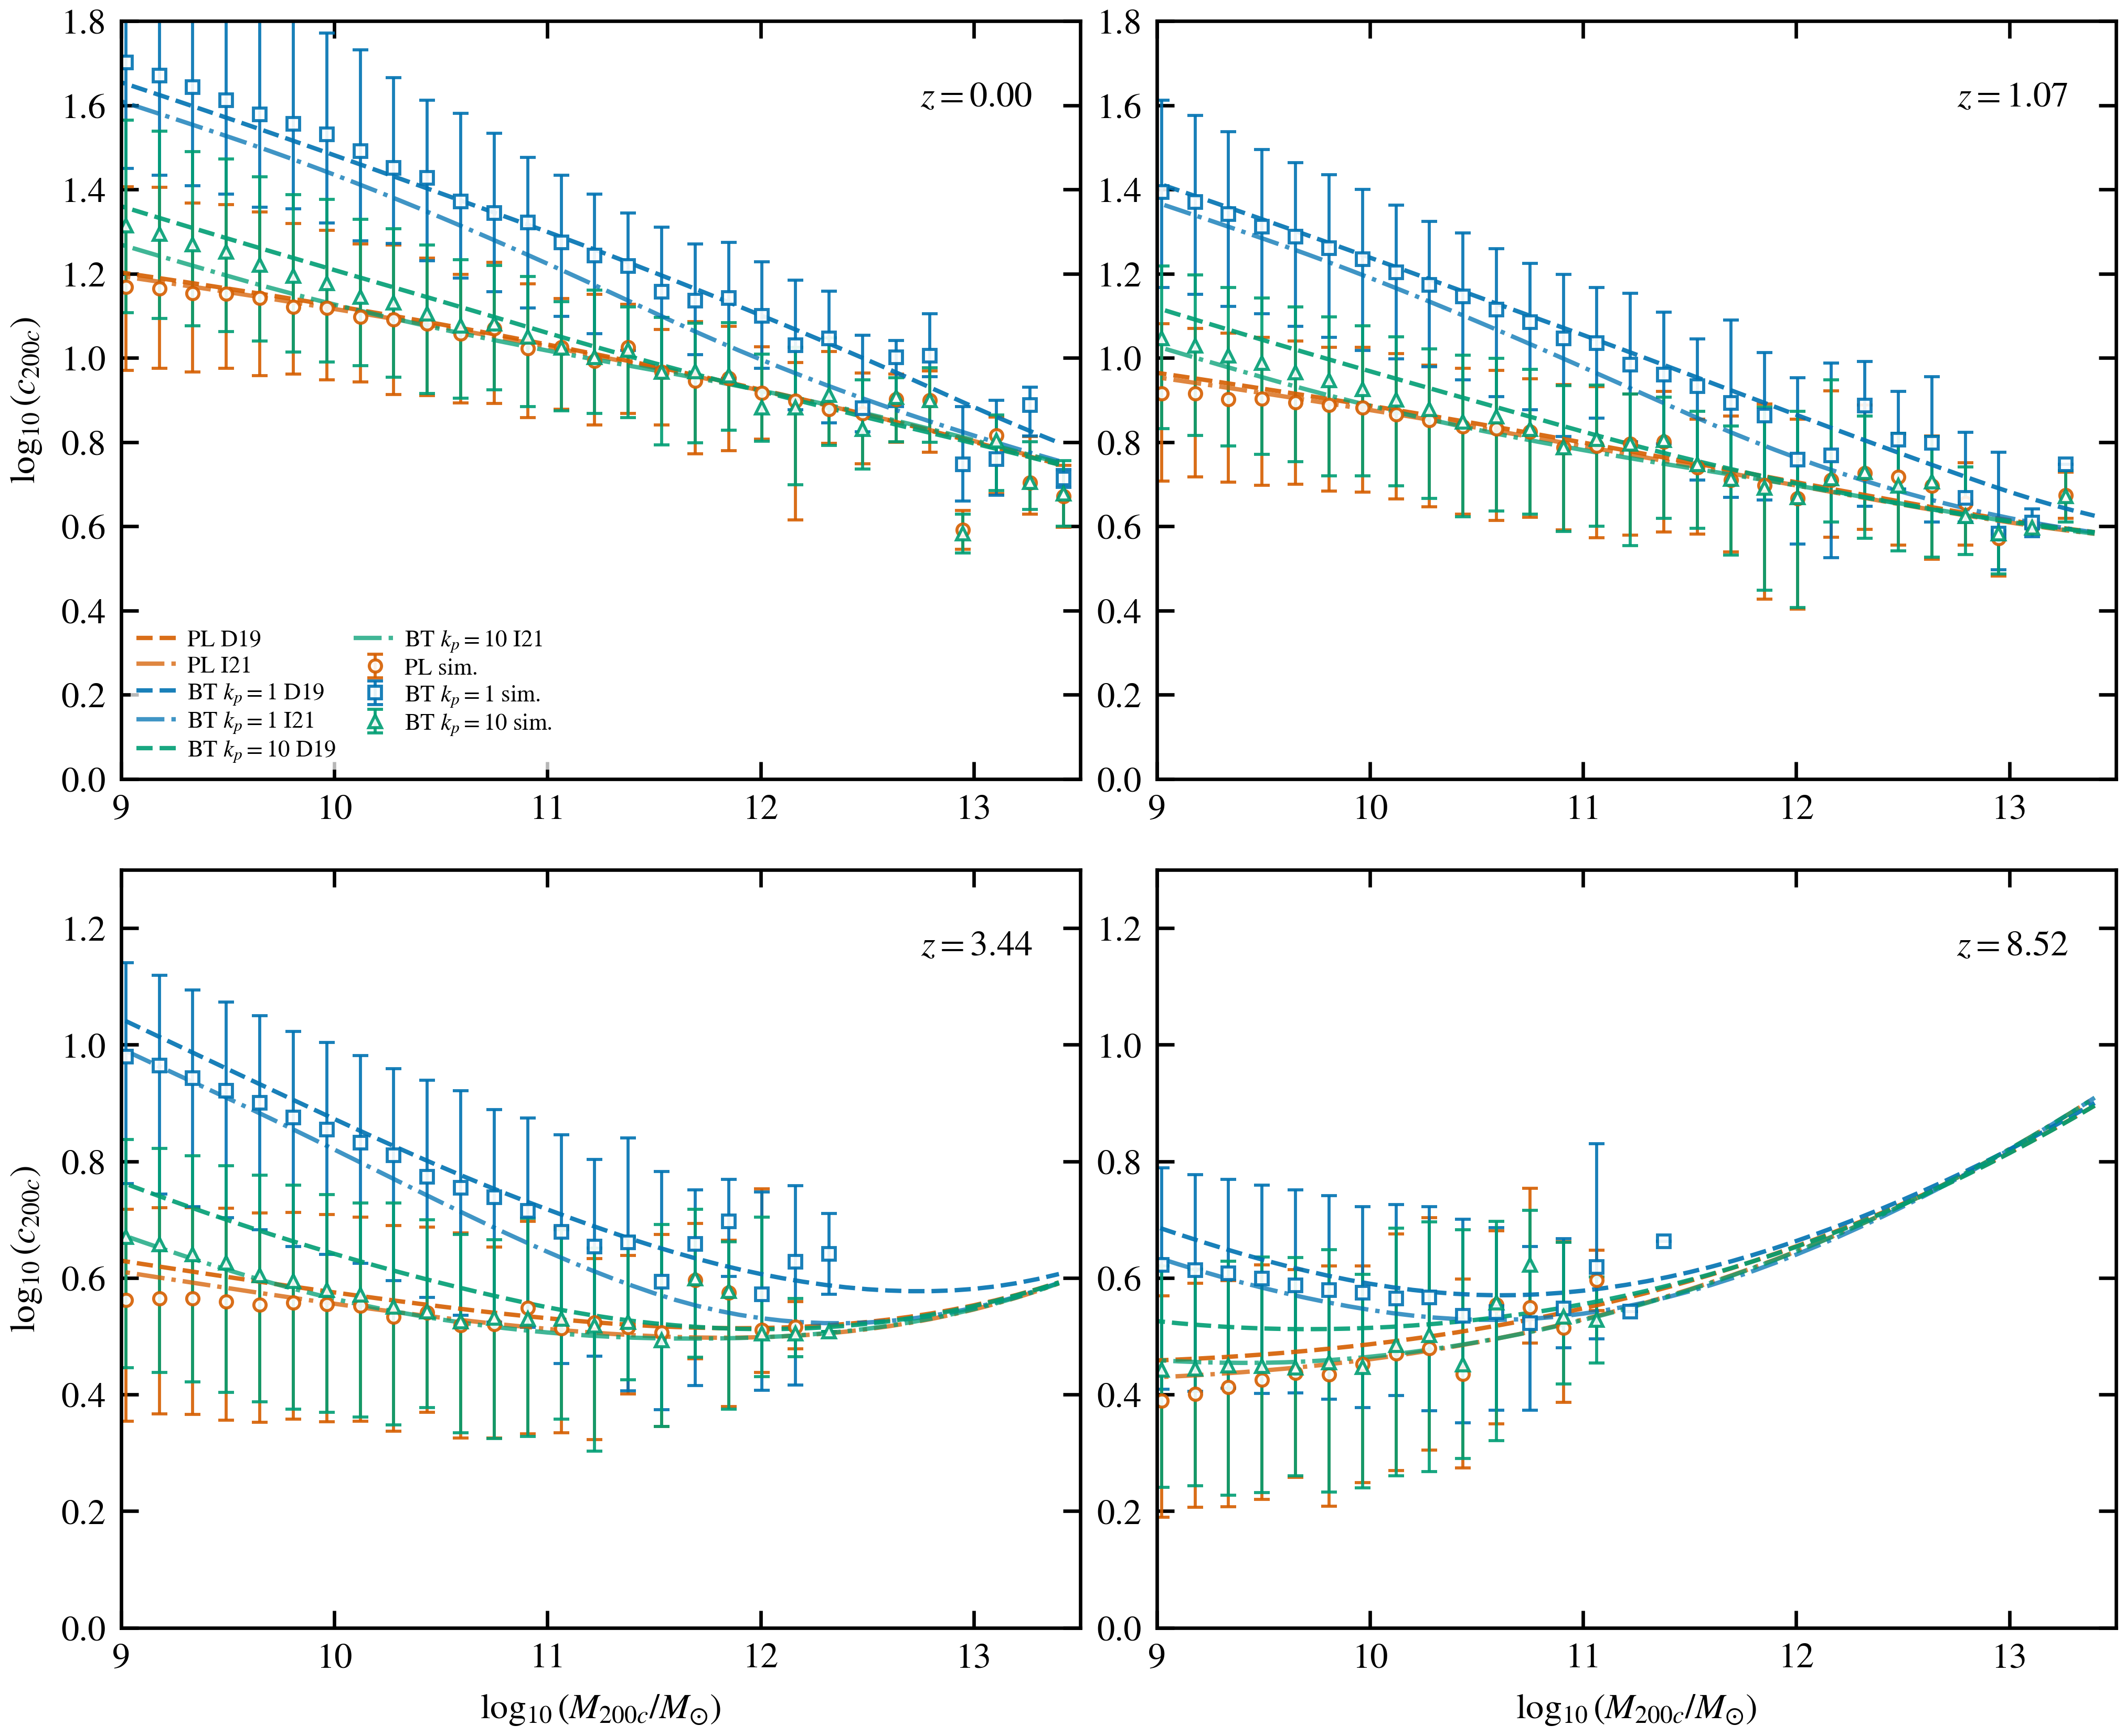
\includegraphics[width=0.92\textwidth,height=0.68\textheight,keepaspectratio]{concentration-qc.png}
    \caption{\blue{Concentration--mass relations for the PL, BT\_soft ($k_p=1\,h\,\mathrm{Mpc}^{-1}$, $m_s=1.5$), and BT\_deep ($k_p=10\,h\,\mathrm{Mpc}^{-1}$, $m_s=1.5$) models at four representative redshifts. Symbols show the simulation measurements and solid curves show the corresponding semi-analytic predictions. The lower panels give the concentration ratios relative to the PL model. At fixed mass, halos in the blue-tilted models are systematically more concentrated, with the strongest differences occurring in the low-mass regime.}}
    \label{fig:concentration_comparison}
\end{figure*}
\fi

We compare the halo concentration-mass relation across four key epochs, from high redshift ($z \approx 8.52$) to the present day ($z = 0.00$), for three distinct cosmological models: the standard Cold Dark Matter (CDM) model (PL), the strongly blue-tilted model (BT, $k_p=1$), and the weakly blue-tilted model (BT, $k_p=10$). The concentration is defined as $c_{200c} = R_{200c} / r_s$, where $R_{200c}$ is the spherical overdensity radius with respect to the critical density and $r_s$ is the scale radius of the NFW profile.

The analysis reveals a clear mass and redshift dependence in the concentration enhancement predicted by blue-tilted models. While all models exhibit the expected anti-correlation between concentration and halo mass, the divergence between the blue-tilted and standard models is most pronounced at low redshift. At $z=0$, the concentration of low-mass halos ($M_{200c} \sim 10^9 M_\odot$) in the strongly blue-tilted model ($k_p=1$) is a factor of 2 to 3 higher than in the standard CDM model. The weakly blue-tilted model ($k_p=10$) also shows significant enhancement, though to a lesser degree. This difference diminishes progressively with increasing redshift.

The redshift evolution of this effect follows a specific pattern: although the concentrations in blue-tilted models remain several times higher than in the standard model even at high redshift ($z \approx 8.52$), the relative magnitude of the divergence is greatest at $z=0$. This trend indicates that the distinct initial conditions set by the blue-tilted power spectrum are subsequently amplified through cosmic time. The nonlinear growth, merger history, and mass accretion processes that dominate structure formation at low redshifts act to solidify and magnify the differences in the internal structure of halos across the models. The ratio curves quantitatively confirm this evolution, showing the highest and steepest profiles (strongly mass-dependent) at $z=0$ and flatter, lower profiles at high redshift.

Theoretical predictions are in good overall agreement with the simulation trends, validating the implementation of the custom power spectra. Residual discrepancies at the high-redshift, low-mass end are likely attributable to simulation resolution limits or simplifications in the analytical concentration model under extreme conditions. The established evolutionary pattern---whereby concentration differences expand with cosmic time and peak at low redshift---provides a distinctive signature of blue-tilted primordial power spectra. It underscores that the impact of enhanced small-scale power is not only imprinted at halo formation but is also systematically leveraged by later nonlinear evolution. Consequently, observational constraints on the concentration of low-mass halos at low redshift will serve as a powerful probe for testing deviations from the standard scale-invariant primordial power spectrum.

\subsection{Power Spectrum\label{subsub:PS}}
The nonlinear matter power spectrum provides a complementary summary of how the modified primordial spectrum propagates through structure formation. In combination with the halo-based statistics above, it directly captures the redistribution of clustering power across scales and redshifts. \blue{Compared with one-point halo statistics, the power spectrum is particularly informative because it measures the cumulative clustering response over a broad range of scales. In blue-tilted models, the enhancement of small-scale primordial fluctuations first appears in the linear regime and is then reprocessed by nonlinear evolution, halo formation, and merger-driven mode coupling. We therefore expect the largest deviations from the PL model at high wavenumber, together with a redshift dependence that reflects the time available for nonlinear amplification. The comparison presented below is intended to test this picture directly and to connect the halo-scale differences discussed above with the global clustering signal of the matter field.}

\begingroup
\color{red}
The nonlinear matter power spectrum is measured directly from the particle distribution in the simulations at the selected output snapshots. Operationally, the dark matter particles are assigned to a regular mesh, the Fourier-space density field is constructed, and the isotropically averaged power spectrum is computed in bins of wavenumber. In a finalized version of the analysis, the precise estimator settings should be documented explicitly, including the mesh size, mass-assignment scheme, shot-noise treatment, and any deconvolution or window-function corrections applied to the raw spectrum. These technical choices affect the quantitative reliability of the spectrum at the highest resolved wavenumbers and therefore need to be stated clearly for reproducibility.

The interpretation of the measured power spectrum also requires a clear statement of its trusted scale range. At small $k$, the finite simulation volume limits the number of independent long-wavelength modes and increases sample variance. At large $k$, force softening, discreteness, and estimator choices can bias the recovered power. The curves shown below should therefore be interpreted as reliable over an intermediate dynamic range whose exact boundaries are determined by the numerical setup. In the final manuscript, we plan to report these adopted scale cuts explicitly and, where appropriate, compare them against convergence-test runs.

From a physical perspective, the power-spectrum statistic provides an important bridge between the halo-based diagnostics and the global clustering field. If the blue-tilted initial condition primarily boosts low-mass halo formation and inner halo concentrations, then one expects a corresponding increase in power at high wavenumber, with a redshift dependence reflecting the growth of nonlinear mode coupling. This makes the power spectrum a particularly useful summary statistic for connecting our simulation results to future weak-lensing and small-scale clustering constraints.
\endgroup

\ifshowfigures
\begin{figure*}[t]
    \centering
    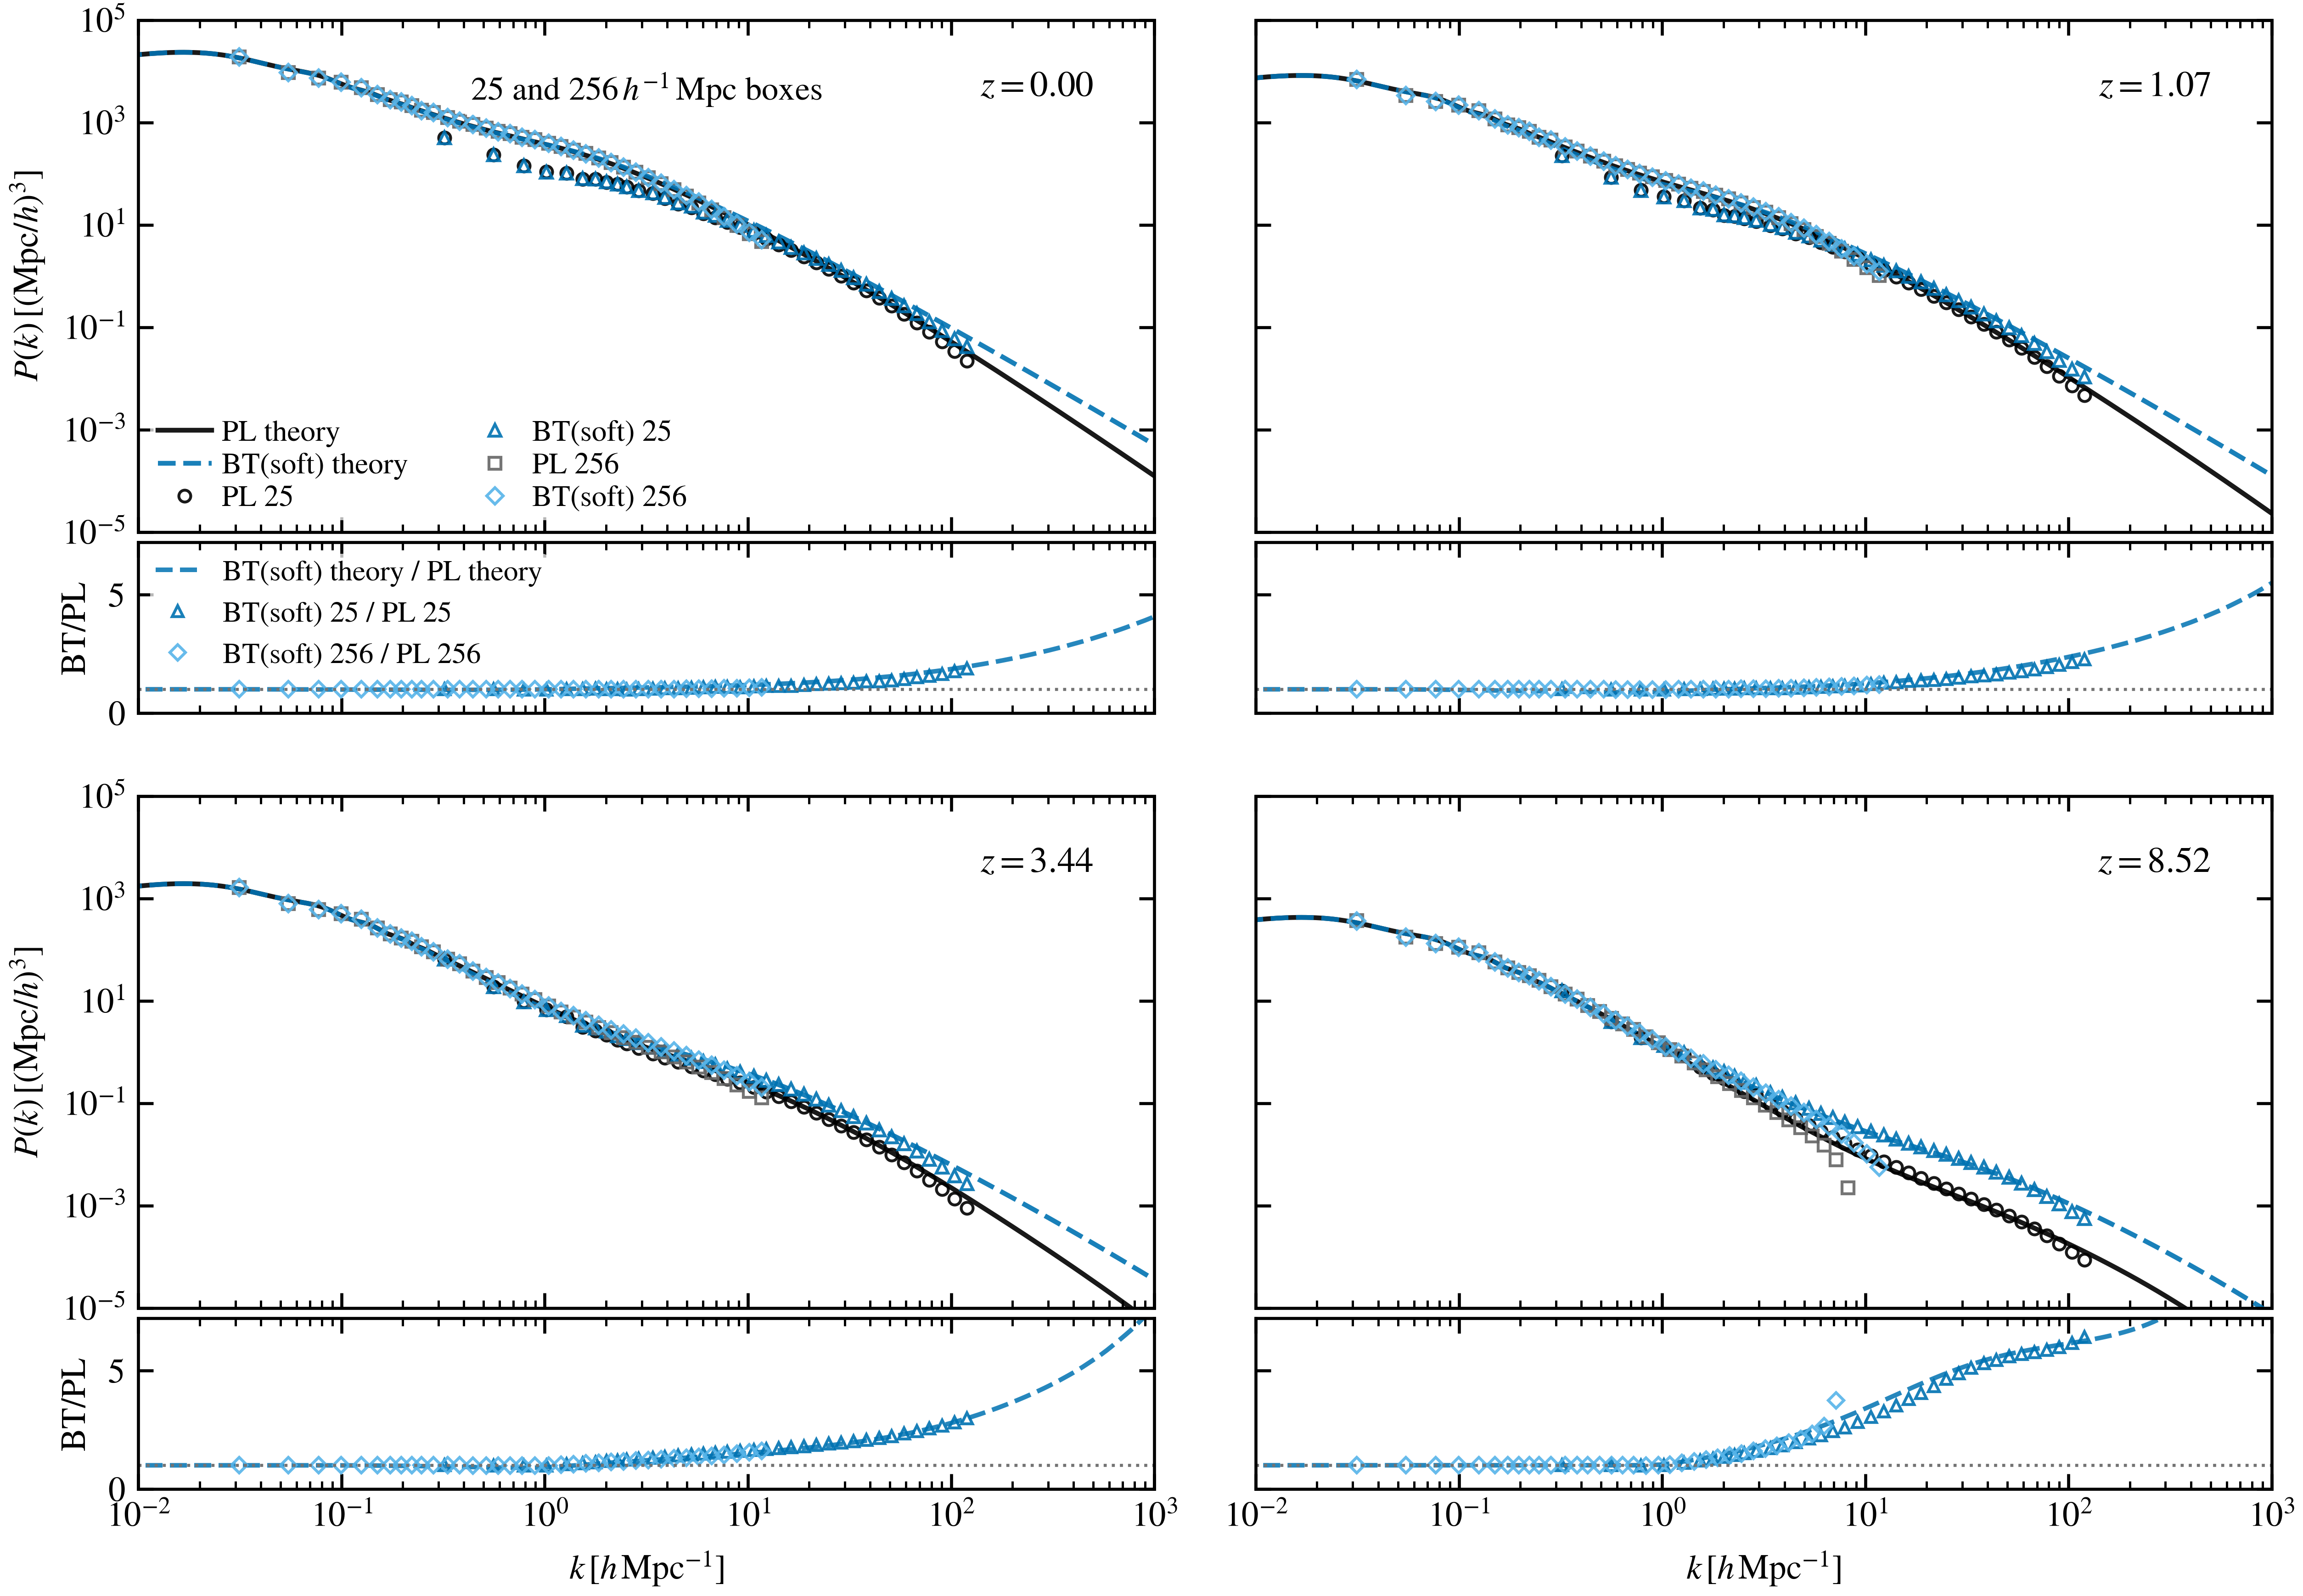
\includegraphics[width=0.92\textwidth,height=0.70\textheight,keepaspectratio]{power-spectrum.png}
    \captionsetup{width=0.92\textwidth}
    \caption{\blue{Nonlinear matter power spectra at $z=0$ for the PL, BT\_soft, and BT\_deep models. The upper panel shows the dimensionless power spectrum $\Delta^2(k)$, while the lower panels give the ratios of the blue-tilted models relative to PL. In both BT cases, the excess primordial small-scale power is converted into an enhancement of nonlinear clustering at large $k$, with the magnitude of the effect depending on the pivot scale of the initial spectrum.}}
    \label{fig:power_spectra_ratio_z0}
\end{figure*}
\fi

\section{Discussion and Limitations}
\label{sec:discussion}

\subsection{Physical Interpretation of the Main Trends}
Taken together, the results in Section~\ref{sec:results} point to a coherent physical picture. Increasing the primordial power on sufficiently small scales raises the initial amplitude of low-mass density perturbations, allowing them to cross the collapse threshold earlier. This earlier collapse naturally produces three related effects: an enhanced abundance of low-mass halos, earlier half-mass assembly times, and denser inner halo structures. The concentration--mass relation and stacked density profiles therefore provide the internal-structure counterpart of the abundance signal seen in the halo mass function.

The nonlinear matter power spectrum gives a field-level view of the same process. The high-$k$ excess is not simply a passive remnant of the input spectrum; it is reshaped by nonlinear gravitational evolution as small structures form, merge, and contribute to clustered matter on progressively larger nonlinear scales. The fact that the halo mass function, assembly histories, halo profiles, concentrations, and nonlinear power spectrum all respond in the same direction supports the interpretation that the measured trends are driven by the modified initial conditions rather than by a single analysis choice.

The impact of the blue-tilted models is also strongly scale- and redshift-dependent. The clearest differences appear in low-mass halos, early epochs, and high-$k$ clustering, while the high-mass end shows weaker sensitivity because rare massive halos form later and are more strongly affected by nonlinear mode coupling. This behavior identifies the observational regime in which small-scale primordial physics is most likely to remain visible: low-mass halo abundance, inner halo structure, and small-scale matter clustering are more sensitive probes than the properties of the most massive halos alone.

\subsection{Relation to Previous Work}
The present study is complementary to recent work that connects modified small-scale primordial power to specific observational probes. Studies motivated by JWST high-redshift galaxy candidates ask whether enhanced small-scale power can increase the abundance of early luminous systems \citep{Parashari23JWSTPPS,Hira24bluetilt}. Our simulations do not model star formation or galaxy selection, but they test the underlying dark-matter prerequisite for that scenario: whether the modified initial spectrum produces more early low-mass structure and shifts halo assembly to higher redshift.

Our work also differs from studies focused on particular environments or observables. Zoom-in simulations of Milky Way--mass systems have examined how blue-tilted initial conditions affect satellite and subhalo populations \citep{Wu25BT}. By contrast, the periodic-box simulations used here are designed to measure population-level statistics and field-level clustering across the full volume. Low-redshift constraints from dwarf-galaxy densities and strong-lensing substructure probe the same broad physics through halo internal structure and sub-galactic matter fluctuations \citep{Dekker25DwarfPPS,Gilman22SubgalacticPPS}; the profile and concentration measurements in this paper provide the corresponding dark-matter-only response before baryonic modeling and selection effects are added.

Finally, 21 cm studies emphasize that cosmic dawn and reionization may provide access to small-scale matter fluctuations that are otherwise difficult to observe \citep{Munoz20SmallScale21cm,deKruijf25DarkAges,Zhu26SKAPPS}. The connection to our results is indirect but important: the halo abundance, assembly-redshift, and nonlinear-power signatures measured here specify which mass scales, redshifts, and wavenumbers are most affected by enhanced primordial power. In this sense, the contribution of the present paper is not to replace observation-specific analyses, but to provide the simulation-level link between the modified PPS and the dark-matter statistics that those analyses rely on.

\subsection{Numerical and Modeling Limitations}
Several limitations should be kept in mind when interpreting the present results. First, all simulations analyzed here are dark-matter-only runs. This choice is appropriate for isolating the gravitational imprint of the primordial power spectrum, but it also means that baryonic processes such as gas cooling, stellar feedback, and reionization are absent. Since these processes can alter halo density profiles, subhalo survival, and the galaxy--halo connection, our results should be interpreted as predictions for the underlying dark matter field rather than as direct predictions for observed galaxy populations.

Second, different summary statistics are limited by different numerical systematics. Halo counts at the low-mass end are affected by particle discreteness and halo-finder thresholds; density profiles and concentrations are sensitive to the innermost resolved radius and centering uncertainties; and the nonlinear power spectrum depends on box size, force resolution, and estimator details. Although the broad trends are consistent across multiple diagnostics, a final publication-quality version of this study should present explicit convergence figures and adopted reliability cuts for every measured quantity.

Third, the theoretical comparisons used in the halo mass function and concentration analyses are intentionally simplified. They are valuable because they provide a controlled baseline tied to the same input linear power spectrum, but they should not be interpreted as exact predictions in the strongly nonlinear regime. Residual discrepancies between simulation and analytic models may therefore reflect both genuine nonlinear physics and the limited calibration range of the fitting formulae employed.

\subsection{Connection to Observations}
An important next step is to translate these simulation-level signatures into observation-facing predictions. The most promising avenues appear to be those that directly probe low-mass structure: high-redshift galaxy number counts, strong-lensing flux anomalies, satellite-galaxy statistics, and weak-lensing measurements of small-scale clustering. Strong-lensing analyses already provide a route to infer the primordial matter power spectrum from the abundance and concentration of low-mass halos on sub-galactic scales \citep{Gilman22SubgalacticPPS}, while dwarf-galaxy central densities can place complementary limits on blue- or red-tilted spectra \citep{Dekker25DwarfPPS}. However, each of these observables introduces additional astrophysical and selection-model uncertainties. The value of the present work is therefore not that it delivers a one-to-one observational constraint already, but that it identifies a physically motivated set of statistics and scale ranges where departures from the standard primordial spectrum are likely to be largest.

In this sense, the main scientific contribution of the paper is to establish a theoretical benchmark for future constraint studies. Once baryonic modeling, survey selection functions, and forward modeling are included, the diagnostics presented here can be mapped onto actual likelihood analyses. Among them, the halo mass function, concentration--mass relation, and nonlinear matter power spectrum appear especially promising because they encode complementary aspects of the same primordial enhancement and can therefore provide cross-validation in future observational work.

\section{Conclusions}
\label{sec:conclusion}
We have used dark-matter-only cosmological $N$-body simulations to study how enhanced small-scale primordial power is mapped into nonlinear structure formation. By comparing a standard power-law primordial spectrum with two blue-tilted benchmark models, we isolated the gravitational response to the modified initial conditions before introducing baryonic physics, galaxy formation, or survey-selection effects.

Our main conclusions are as follows. First, the blue-tilted models produce a clear excess of low-mass halos, with the largest relative differences appearing at high redshift and at the low-mass end of the halo mass function. This confirms that enhanced small-scale primordial power accelerates the collapse of small structures. Second, halos in the blue-tilted simulations assemble earlier: at fixed final mass, their half-mass assembly redshifts are shifted upward relative to the standard model. Third, the internal structure of halos is modified in a consistent way. The stacked density profiles are denser in the inner regions, and the concentration--mass relation is systematically elevated, especially for low-mass halos. Fourth, the nonlinear matter power spectrum retains a pronounced high-$k$ enhancement, showing that the primordial excess is amplified and redistributed by nonlinear gravitational evolution.

These results provide a simulation-level benchmark for interpreting observational probes of small-scale primordial power. The same physical changes that appear in the simulations--more abundant low-mass halos, earlier assembly, denser inner structures, and enhanced high-$k$ clustering--are directly relevant to JWST high-redshift galaxy counts, strong-lensing substructure constraints, dwarf-galaxy structure, 21 cm forecasts, and future small-scale clustering measurements. At the same time, our results should not be interpreted as direct observational constraints, because baryonic physics and selection effects have not yet been included.

Future work should therefore connect the present dark-matter-only benchmarks to forward models of specific observables. The most important extensions are hydrodynamic simulations or semi-analytic galaxy modeling for high-redshift galaxies, explicit reionization modeling for 21 cm predictions, and larger simulation suites that can quantify convergence and sample variance across the relevant mass and wavenumber ranges. Such extensions will make it possible to test whether enhanced small-scale primordial power is merely allowed by current data or actually favored by a joint analysis of multiple small-scale probes.




% ====== acknowledgments ====== %

\section*{Acknowledgments}
\begingroup
\color{red}
We will acknowledge funding support, computational resources, and relevant collaborative discussions in the final version of the manuscript. In particular, this section should specify the computing facilities used for generating the initial conditions, evolving the simulations, and carrying out the post-processing analysis.
\endgroup



% ====== bib ====== %
\bibliographystyle{apsrev4-1-JHEPfix}
\bibliography{main}

%\printbibliography

\clearpage

\appendix

\section{Additional Numerical Details}
\begingroup
\color{red}
This appendix can be used in the final manuscript to collect technical material that supports, but would otherwise interrupt, the flow of the main text. Natural candidates include: the explicit implementation details of the modified primordial power spectrum in the initial-condition generator and in the custom \textsc{Colossus} modules; additional convergence plots for the halo mass function, density profile, concentration--mass relation, and nonlinear matter power spectrum; and tables summarizing the adopted trusted mass, radial, and wavenumber ranges for the main analyses.
\endgroup

\end{document}
